\chapter{Garbage Collection}\label{chapter:garbage-collection}

\definecolor{compilergray}{HTML}{7D7F85}
\newcommand{\compilergen}[1]{\texttt{\textit{\textcolor{compilergray}{#1}}}}

\newcommand{\gcblock}[2]{
\node[draw,fill=darkest,fill opacity=0.05,minimum width=2.2cm,minimum height=1cm] 
  (#1) at #2 { };
\draw ($(#1.north west) + (0.2cm,0)$) -- ++ (0,-1cm);
\draw ($(#1.north west) + (1.2cm,0)$) -- ++ (0,-1cm);
\draw (#1.west) -- ++ (0.2cm,0);
}

\newcommand{\rcblock}[3]{
\node[draw,fill=darkest,fill opacity=0.05,minimum width=2.4cm,minimum height=0.8cm] 
  (#1) at #2 { };
\draw ($(#1.north west) + (0.8cm,0)$) -- ++ (0,-1cm);
\draw ($(#1.north west) + (1.8cm,0)$) -- ++ (0,-1cm);
\node[anchor=south west,minimum width=0.8cm,minimum height=0.8cm,fill=highlight,fill opacity=0.1] at (#1.south west) {};
\node at ($(#1.west) + (0.4cm,0)$) { \large\color{darkest}\bfseries{#3} };
}

\newcommand{\copyblock}[2]{
\node[draw,fill=darkest,fill opacity=0.05,minimum width=2.2cm,minimum height=1cm] 
  (#1) at #2 { };
\draw ($(#1.north west) + (0.2cm,0)$) -- ++ (0,-1cm);
\draw ($(#1.north west) + (1.2cm,0)$) -- ++ (0,-1cm);
}
\newcommand{\forwardedblock}[2]{
\node[draw,dashed,highlight,minimum width=2.2cm,fill opacity=0.1,fill=highlight,minimum height=1cm] 
  (#1) at #2 { };
\draw[highlight,dashed] ($(#1.north west) + (0.2cm,0)$) -- ++ (0,-1cm);
\draw[highlight,dashed] ($(#1.north west) + (1.2cm,0)$) -- ++ (0,-1cm);
}
\newcommand{\markBlock}[1]{
\draw[draw=darkest,fill=black] (#1.south west) rectangle ++(0.2cm,0.5cm);
}
\newcommand{\fieldOne}[1]{($(#1.east) + (-1.5cm,0)$)}
\newcommand{\fieldTwo}[1]{($(#1.east) + (-0.5cm,0)$)}

\newcommand{\highlightBlock}[1] {
  \node[fill=yellow,fill opacity=0.3,
  minimum width=2.6cm,minimum height=1.4cm,anchor=north west] at
   ($(#1.north west) + (-0.2cm,0.2cm)$) { };
}

\newcommand{\collectBlock}[1] {
  \node[fill=background,fill opacity=0.85,
  minimum width=2.6cm,minimum height=1.4cm,anchor=north west] at
   ($(#1.north west) + (-0.2cm,0.2cm)$) { };
}

\section{Overview}
We have completed our tour of the front and middle ends of a compiler, compiling \texttt{Slang} into an intermediate representation.

\texttt{Slang} is a good first language for teaching compilers because it is relatively simple, making compilation easier. The compiler we've built is also straightforward. In contrast, more complex languages like \texttt{OCaml}, \texttt{Java}, and \texttt{C} have more advanced features, and their compilers often do more than what we've covered. In these next chapters, we’ll explore how these more advanced languages and compilers differ.

Our first topic is garbage collection, which involves automatic memory management, a feature that more complex languages require their compilers to support efficiently.

\subsection{Manual Memory Management}
In \textsf{Part IB C and C++}, you got to work with manual memory management, using \texttt{malloc}, and \texttt{free}. We hope you understood that freeing memory is important. We have a finite amount of space on the heap, and we need to free memory in order to avoid running out. More importantly, we hope you got to grips with managing memory manually, and know how to build programs that allocate and free memory precisely when they should. 

\textit{Most} importantly, we hope that you absolutely hated the experience and never want to have to manage memory yourself. While manual management of memory gives you a lot of control, it is also extremely error-prone. There are three types of bugs: missing free, double-free, and use after free.

\begin{figure}[H]
    \centering
    \import{figures}{manual-memory-management}
    \caption{Problems arising from manual memory management}
    \label{fig:manual-memory-management}
\end{figure}

Note that \textit{freeing} memory is a lot harder than \textit{allocating} memory.

This motivates the need for \textit{automatic} memory management. We want our programming language to offer the ability to manually \textit{allocate} space on the heap, but \textbf{not} (or at least, not require) the ability to manually \textit{free} space on the heap.

Lots of programming languages allow for this. For example, we can allocate a dictionary on the heap in \texttt{Python}

\begin{minted}[bgcolor=backcolour]{Python}
d = {"x": 3, "y": 4}
\end{minted}
Or \texttt{OCaml}
\begin{minted}[bgcolor=backcolour]{Python}
let d = [("x", 3); ("y", 4)]
\end{minted}
Without needing to specify when and where to free this dictionary.

Of course, \texttt{Java} is another language with automatic memory maangement, and indeed you will have learnt about garbage collection in \textsf{Part IA Object-Oriented Programming}.

\subsection{Automatic Memory Management}
We have motivated the need for automatic memory management.

In slightly more detail, garbage collection automatically \textit{identifies} and \textit{frees} heap-allocated objects that are no longer in use. 

In this chapter, therefore, we will take you through various algorithms that automate the process of identifying and freeing garbage.

At a high level, we will also consider two important aspects of garbage collectors: \textit{correctness} and \textit{performance}. These correspond somewhat to the \textit{safety} and \textit{liveness} properties you learnt about in \textsf{Part IB Concurrent and Distributed Systems}.

A correct garbage collector is \textit{safe}: it never collects anything that is not actually garbage, i.e. anything that the program still needs.

A performant garbage collector is an elusive creature. The general idea is one of \textit{liveness}: it clears space for the program to do work. But the garbage collector itself needs space and time, and it can't take up too much of either! Defining the \textbf{metrics} by which performance is measured is thus really important -- do we care about latency, or throughput, or space? Do we care about average-case or worst-case guarantees? Are we testing on representative programs? 

Garbage collection is therefore one of the areas of compilers that lives closest to the statistical branch of computer science: your skills from \textsf{Part IB Data Science} will come in handy here.

\subsubsection{The Garbage Collection Perspective}
Garbage collection offers an interesting perspective on programs. In garbage collection, the garbage collector is primary, and the program is secondary. The program is seen as a pesky creature that mutates memory and gets in the way of the work of the garbage collector, plus a demanding creature that consumes an incredible amount of resource. Indeed, in the garbage collection literature, the program is called the \textit{mutator}.

\subsubsection{Research Directions}
Garbage collection remains an active research area. Its continued relevance is the result of three trends. 

First, especially with the hype around machine learning, the nature of the compute is changing to use ever-larger data sets, which place greater demands on memory utilisation. 

Second, over the last few decades, CPU speed improvements have significantly outpaced memory speed improvements (as you will learn in \textsf{Part II Advanced Computer Architecture}). For example, \Cref{fig:memory-vs-cpu-speed}, taken from \citet{hennessy-patterson-2017} (Chapter 5, Page 289), illustrates how improvements to CPU speed have significantly outpaced memory speed. Since CPU speed has increased, so too has the rate at which programs can perform allocation. Since memory speed has not kept up, garbage collectors have to work even harder to be performant. Specifically, locality and cache usage play a large role in collector design.

\begin{figure}
    \centering
    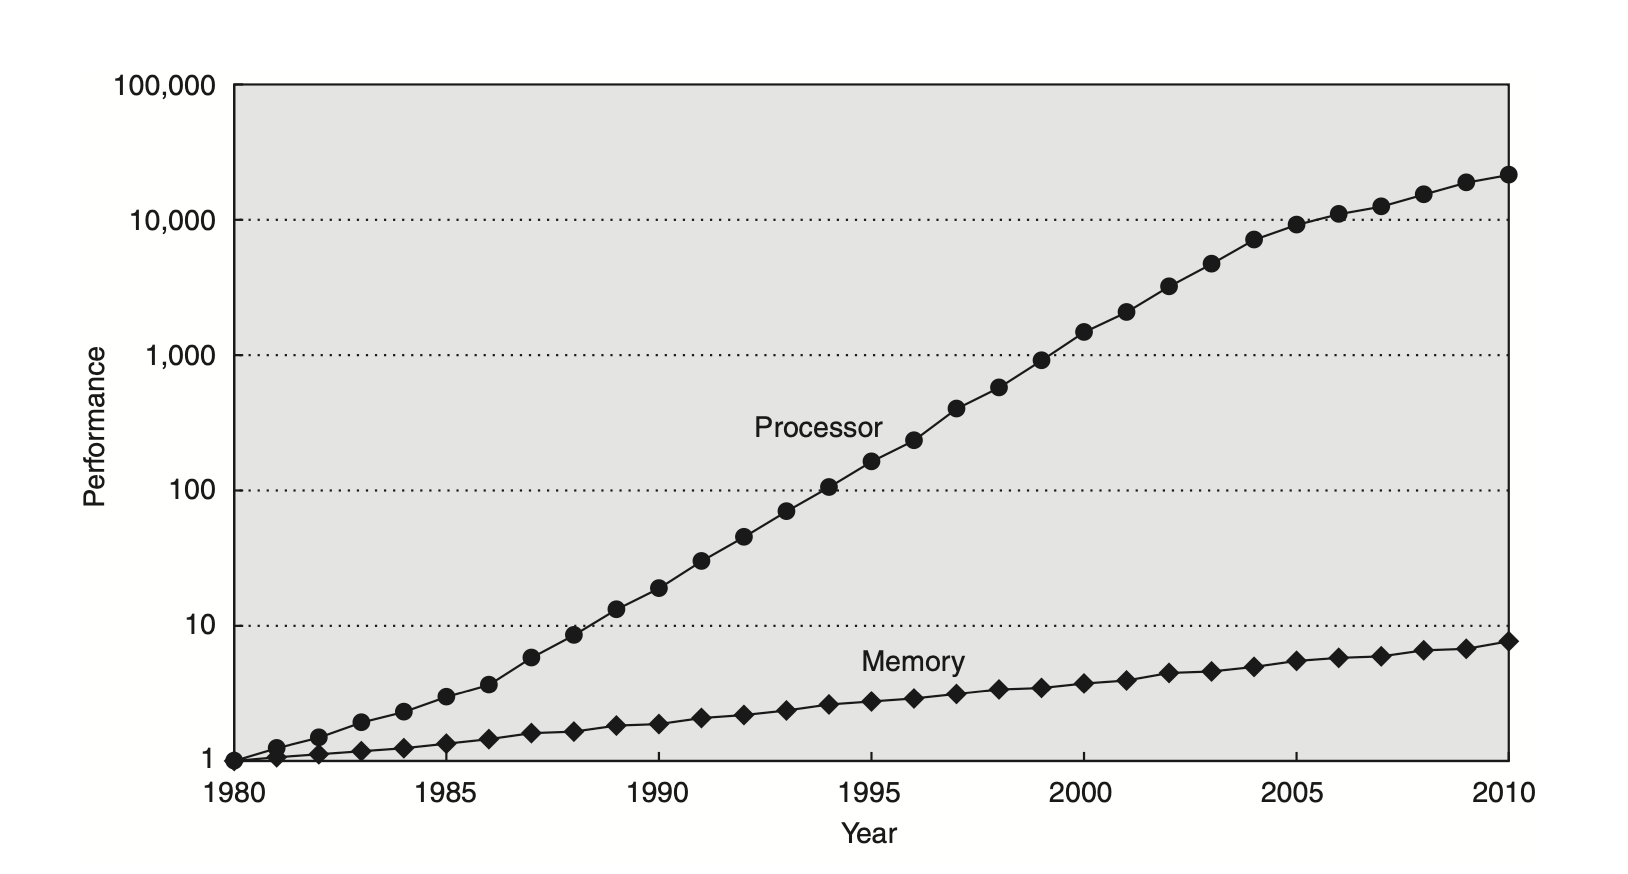
\includegraphics[width=0.8\linewidth]{lec12/figures/hennesy-patterson.png}
    \caption{A figure from \citet{hennessy-patterson-2017}, illustrating how CPU speed improvements have outpaced memory speed improvements. Note the logarithmic scale.}
    \label{fig:memory-vs-cpu-speed}
\end{figure}

Third, ever since the breakdown of Dennard Scaling in the 2000s (\textsf{Part IB Introduction to Computer Architecture}), we have seen a move towards multi-core architectures that exploit thread-level parallelism. This increases the relevance of concurrent (same core, different thread), or parallel (different core, different thread) approaches to garbage collectors. 


\section{Approximating Garbage}
Our key goal is to automatically identify when a heap-allocated object is garbage, or no longer in use.

Unfortunately, it is not possible to build an algorithm that automatically determines if a heap allocated object is no longer in use. It is incredibly simple to come up with a counter example:

\begin{minted}[bgcolor=backcolour]{Python}
let d = [("x", 3); ("y", 4)]
if f halts on a then
   d
\end{minted}
Whether \texttt{d} is still in use depends on if \texttt{f} halts on \texttt{a}. There is no algorithm that can decide if \texttt{f} halts on \texttt{a} for all \texttt{f}, \texttt{a} (c.f. \textsf{Part IB Computation Theory}).

If this is impossible, how then do garbage collection algorithms work? The identification of garbage collection algorithms is fundamentally based on an \textit{approximation}. 

Recall that the heap is not directly accessible, but must be accessed via \textit{pointers}. These pointers can live in various places -- such as registers, global variables, and the stack. In order for a heap object to be accessible, it \textit{must} be reachable via some chain of pointers that starts at the root set.  

\begin{figure}
    \centering
    \import{figures}{reachability-from-root-set}
    \caption{Reachability from a root set, a safe under-approximation of garbage}
    \label{fig:reachability-from-root-set}
\end{figure}

This leads to a \textbf{syntactic} definition of ``in use''. This definition is based on reachability: a heap object $H$ is no longer in use if it cannot be reached from the root set. Define a predicate, \texttt{unreachable}, that tells you for each heap object if it is unreachable from the root set. We say a heap object $H$ is (syntactically) garbage if \texttt{unreachable}$(H)$.

This syntactic definition contrasts against the \textit{semantic} definition of garbage, which is ``will never be de-referenced by the program''. Imagine we had some oracle, some ground truth predicate, that could tell us when this semantic property holds. Call this semantic predicate \textsf{garbage}$(H)$.

We now state the safety property. To be safe, whenever something is unreachable, it must be garbage. The inverse need not be true: just because something is reachable does not mean that it is not garbage, since being ``in reach'' and being ``used in the future'' are not equivalent. Therefore, we write
\[\texttt{unreachable}(H) \implies \textsf{garbage}(H) \]
Equivalently, we say the set of \texttt{unreachable} objects must under-approximate the set of \textsf{garbage} objects. 

This idea of safe under-approximation (or over-approximation, depending on how you choose to measure it) is a recurring theme in static analysis (although in this case, the analysis is dynamic)! You will see many more examples in \textsf{Part II Optimising Compilers}. The key idea is that almost everything we care about is undecidable, in exactly the same way whether something is garbage or not is undecidable. Therefore, \textbf{safe} approximation is the best we can do.

\subsection{Representations for Garbage Collection}
In order to \textit{compute} \texttt{unreachable}, we need to answer two questions: First, when do we have a pointer? Integers and pointers can often look very similar. since we care about tracing pointers, we need to know \textbf{which} it is. 

Second, once we've followed a pointer, we'll end up with some object on a heap. Objects come in many different shapes and sizes. How do we know if our object is a pair of two values, or a megabyte long array? We need to know how large the object is, and, if we want to continue tracing pointers, a little bit about its internal structure.

\subsubsection{Differentiating between pointers and integers}
\begin{figure}[H]
    \centering
    \import{figures}{integer-tag}
    \caption{Using a tag bit to differentiate between integers and pointers}
    \label{fig:integer-tag}
\end{figure}
To differentiate between pointers and integers, one strategy is to use a \textit{tag} bit to differentiate integers and pointers. For example, in \texttt{OCaml}, integers are 63 bits long. The least significant bit is always set to 1, to indicate that it is an integer. In contrast, pointers are also 63 bits long, but their least significant bit is always set to zero. This makes it easy to test if a value is an integer or a pointer. The test is:
\[\texttt{x \& 1}\]
This can be done very efficiently on most architectures. However, this does come at a cost, which is that arithmetic operations become slightly more expensive. For example,  $x+y$ has to be translated to $x+y - 1$, and $x * y$ has to be translated to $(x >> 1) * (y-1) + 1$.

More information can be found on \href{https://blog.janestreet.com/what-is-gained-and-lost-with-63-bit-integers/}{Jane Street's Tech Blog}.

\subsubsection{Object Representation}
\begin{figure}[H]
    \centering
    \import{figures}{object-representation}
    \caption{Objects typically use headers that carry sizes, among other metadata}
    \label{fig:object-representation}
\end{figure}

In order to ensure the garbage collector has the information it needs about each object on the heap, we typically design compilers that give objects headers. This header carries sizes and other metadata, like the type of the object. 

\subsubsection{Conservative Garbage Collection\optional}
\textit{This section is based on \href{https://dl.acm.org/doi/10.1145/155090.155109}{Space Efficient Conservative Garbage Collection}, by} \citet{boehm-1993}.

Some languages were not designed with garbage collection in mind, and therefore one cannot guarantee that (a) we will be able to distinguish between integers and pointers, and (b) that every object on the heap will have a header that tells us about the shape of the object. Examples of such languages include \texttt{C} and \texttt{C++}. 

Recall, for example, that in \texttt{C} and \texttt{C++}, unless you as the programmer are disciplined enough to do it, sizes of arrays will not be recorded. Thus, you can iterate past the end of an array. Further, you can type-cast integers to pointers, and vice versa, so it can be extremely difficult to tell when something is, or is not, a valid pointer. 

In such cases, we can \textit{still} use garbage collection, but we have to work harder to be safe. Specifically, if the garbage collector cannot tell if a value is an integer or a pointer, it \textit{has} to classify it as an integer. We call such garbage collectors \textit{conservative}, since they are ``risk-averse''. Concretely, in \texttt{OCaml}, the language guarantees that we can determine exactly when something is a pointer, and when something is not a pointer. In contrast, in \texttt{C}, the best our garbage collector can do is determine if something is definitely a pointer, or may be an integer. 

Conservative garbage collectors are generally less performant than its non-conservative cousins, for two reasons. First, because they are less effective at approximating garbage.

Second, because the test for whether something is garbage tends to be a lot less efficient. Often, we need to analyse the bit-pattern to determine if something is or is not a pointer. A range of techniques can be used for this, including

\begin{enumerate}
    \item Heap Size. If the heap is in the range $[a, b]$, and the value is less than $a$ or greater than $b$, then it must not be a pointer.
    \item Alignment. If the allocator maintains an alignment invariant: for example, it will always allocate at a memory address that is some multiple of 8, then if a value is not a multiple of 8, we can determine that it is definitely \textit{not} a pointer.
\end{enumerate}

Assuming we have complete control over allocation (i.e. the user is not allowed to manually perform allocation), we can do better via the technique of a \textbf{blacklist}. The idea is that the garbage collector can proactively blacklist addresses, such that they will never be pointed to. This strengthens our approximation on when something is definitely not a pointer. It works as follows: if the garbage collector finds a value $p$ that is not a pointer but could be allocated as one, and $p$ is ``in the vicinity of the heap'' (i.e. the first technique is likely going to stop being useful, because the heap will grow), then we add $p$ to a blacklist, and prevent memory from ever being allocated at $p$. We can thus conclude forevermore that $p$ is definitely not a pointer. 

For this technique to be effective, we need to perform garbage collection at very frequent intervals, including one right after program start-up, when the heap is still very small. This ensures we capture as many such $p$ as possible. 

Such techniques reveal a tension: the more thorough our analysis of the bit pattern, the better our garbage collector will be at collection. However, such thorough analysis requires (a) more frequent garbage collection, which reduces program throughput, and (b) increases garbage collector latency.

Conservative garbage collectors, despite being less efficient than their non-conservative counterparts, are still incredibly important, especially since many programming languages support calling external libraries written in \texttt{C} or \texttt{C++}. You can find a more thorough evaluation of Conservative Garbage Collectors at \href{https://www.hboehm.info/gc/conservative.html}{Why Conservative Garbage Collectors?}

\section{Two Approaches to Garbage Collection}
We have given a brief overview of how garbage collection works: by computing a reachability set. In a setting where performance is so critical, however, we should investigate how to compute \texttt{unreachable}, and analyse the algorithms from a performance perspective. We shall consider two main approaches: reference counting, and tracing collectors.

\begin{center}
    \import{figures}{rc-vs-tc}
\end{center}

\section{Reference Counting}
In a reference counting approach, we maintain, with each object, a count of the number of pointers to the object (the eponymous \textit{reference count}). An object is unreachable when its reference count reaches zero. The algorithm therefore considers four cases

\begin{center}
    \import{figures}{reference-counting}
\end{center}

Examples of languages that use reference counting include \texttt{CPython} and \texttt{Swift}.

\subsection{Advantages of Reference Counting}
There are three advantages to reference counting. 

First, it is relatively simple to implement. 

Second, it is very space efficient. It requires, at most, several bits per object for the reference count (and objects tend to be much larger than several bits).

Third, in theory, unreachable garbage can be collected \textit{as soon as} the reference count drops to zero. This property is known as \textbf{precision}, but most practical applications of reference counting do not meet this lofty goal. The problem is that ``most implementations tie reference counting to their lexical scope, [and so] retain memory longer than [necessary]'' \cite{reinking-2021}. For example, consider 

\begin{minted}[bgcolor=backcolour]{Koka}
fun foo(){
  val xs = list(1, 1000000) // creates a large list
  val ys = map(xs, inc) // increment each element
  print(ys)
}
\end{minted}
Many compilers will decrease the reference counts of \texttt{xs} and \texttt{ys} as we exit the function body. This retains \texttt{xs} for longer than necessary. 
\begin{minted}[bgcolor=backcolour, escapeinside=!!]{Koka}
fun foo(){
  val xs = list(1, 1000000) // creates a large list
  val ys = map(xs, inc) // increment each element
  print(ys)
  !\compilergen{drop(xs)}! // compiler generated
  !\compilergen{drop(ys)}! // compiler generated
}
\end{minted}
In the listing above, the \compilergen{grey} colour indicates compiler generated code. \texttt{drop} is a function that decrements the reference count, and, if it reaches zero, frees the object.

\subsection{Disadvantages of Reference Counting}
Reference Counting suffers from several drawbacks: cycles, chains, and (poor interaction with) concurrency.

\subsubsection{Cycles}
Reference counting cannot collect cycles.

\begin{center}
    \import{figures}{rc-cycles}
\end{center}

Even though there are no other references to these objects in the program, ergo, these objects are not reachable from the root set, they will never be collected.

\subsubsection{Chains}
In (naïve) reference counting, reclaiming an object can set off an unboundedly large chain of reclamations.

\begin{center}
    \import{figures}{rc-chain}
\end{center}

This means we have very poor guarantees on the worst-case latency of reference counting.

\subsubsection{Concurrency\optional}\label{section:coalesced-reference-counting}
As a final note, (naïve) reference counting turns reads into writes (since the references must be updated). This is a significant problem for concurrent programming (multiple threads on the same core or multiple cores). 

You might remember from \textsf{Part IB Concurrent and Distributed Systems} that you can never be certain when control will switch from one thread to another. The interaction between this non-determinism and non-atomic operations creates race conditions, resulting in bugs. This complicates the design of reference counting in a concurrent setting. In many reference counting implementations, we need to use expensive atomic operations like compare-and-swap to update the reference counts.

In multi-core settings, reference counting can also put more pressure on the cache coherence scheme (\textsf{Part IB Introduction to Computer Architecture}), since reads have turned into writes, so reads to an object must be broadcasted to other cores.

However, the problems of concurrency can be mitigated using a coalesced reference counting scheme. The idea with coalesced reference counting is actually incredibly simple. Your traditional understanding of reference counting is that, as the program executes, it updates the reference counts. If a reference count falls to zero, then we (effectively) switch immediately to the collector, which reclaims the memory instantaneously.

That is \textbf{not} the style of a coalesced reference counter. During program execution (an ``epoch''), threads are not allowed to directly update the reference counts, but instead record increments and decrements to be applied later. For example, if we increment and then decrement a reference count for \texttt{x}, we will push \texttt{INC(x)} and \texttt{DEC(x)} onto a list. If there are multiple threads, each thread will maintain its own list, and will only ever see its own list. An epoch ends when the garbage collector is scheduled to run. The collector is the \textbf{only} thread that has the power to update reference counts. When it runs, it will look at all these lists, among all threads, and \textit{coalesce} the queued updates into a single update. Further, the collector is non-concurrent: it decides when control is handed back to the program. Since the collector is non-concurrent, and it is the only one that can update the reference counts, there are no issues with concurrency. 

Further, we coalesce the writes to the reference counting field into a single write, amortising the cost of many updates over an epoch. You can consult \href{https://www.cs.purdue.edu/homes/hosking/690M/p92-bacon.pdf}{Java without the Coffee Breaks} for more details.

\subsection{Practical Applications of Reference Counting\optional}
\textit{This section is based on \href{https://www.microsoft.com/en-us/research/uploads/prod/2020/11/perceus-tr-v1.pdf}{Perceus: Garbage Free Reference Counting with Reuse} by} \citet{reinking-2021}

Despite the drawbacks of reference counting, its advantages, if they can be realised, are tantalising.

\textit{If} precise reference counting can be implemented, then because of the minimal space overhead, reference counting can be good for systems with very limited memory. 

In this section, we'll take a look at two practical implementations of reference counting, one in \texttt{Koka} and one in \texttt{Swift}. 

First, we'll look at a reference counting implementation in \texttt{Koka}. \texttt{Perceus} is a reference counting algorithm for \texttt{Koka} that achieves precise reference counting. 

Before we get on to the clever bits, let's just see, practically, how basic reference counting is implemented. Assume that we have built-in functions \texttt{incref}, for increasing the reference count of an object, \texttt{decref}, for decreasing the reference count, and \texttt{is-unique}, for determining if the reference count is one. From this, we build two functions, \texttt{dup} and \texttt{drop}, that are called when a resource is \textit{duplicated} by some consumer, and when a resource is \textit{dropped} by a consumer.

\begin{code}[\texttt{dup}: a function that duplicates a resource for a consumer]
\label{code:reference-count-dup}
\begin{minted}[bgcolor=backcolour]{Koka}
fun dup(x){
  incref(x); x
}
\end{minted}
\end{code}

\begin{code}[\texttt{drop}: a function that drops a resource for a consumer]
\label{code:reference-count-drop}
\begin{minted}[bgcolor=backcolour, escapeinside=!!]{Koka}
fun drop(x){
  if is-unique(x) then !\textit{recursively call drop on children}!; free(x)
  else decref(x)
}
\end{minted}
\end{code}

Now onto the clever stuff: \texttt{Perceus} achieves precise reference counting -- objects are garbage collected as soon as they are no longer needed. The authors call this ``garbage free''. Further, when objects are freed, the memory can be immediately re-used. In effect, this allows one to write functional code that compiles down into in-place updates. The authors call this a ``functional but in-place'' paradigm. Finally, the authors use \texttt{Koka}'s language features to deal with cycles and concurrency.

\subsubsection{Precise Reference Counting}
First, \texttt{Perceus} achieves precise reference counting. Let's consider, once again, the imprecise reference counting code. 

\begin{code}[Pseudocode illustrating imprecise reference counting. \texttt{xs} and \texttt{ys} are both in memory simultaneously.]
\label{code:reference-count-base}
\begin{minted}[bgcolor=backcolour, , escapeinside=!!]{Koka}
fun foo(){
  val xs = list(1, 1000000) // creates a large list
  val ys = map(xs, inc) // increment each element
  print(ys)
  !\compilergen{drop(xs)}! // compiler generated
  !\compilergen{drop(ys)}! // compiler generated
}
\end{minted}
\end{code}
The inefficiency arises because the \texttt{foo} function is responsible for freeing \texttt{xs}. \texttt{Perceus} takes an alternative approach -- the ``ownership'' of the \texttt{xs} reference is passed to the functions that \textit{consume} \texttt{xs} (in this case, only the \texttt{map} function). Updating the reference count of \texttt{xs} becomes the responsibility of these consumers, and thus it will be \textit{a} consumer that is responsible for freeing it. 

We thus need to insert functions that alter the reference count of \texttt{xs} in the \texttt{map} function. In the \texttt{Perceus} paper, this is known as \texttt{dup}/\texttt{drop} insertion. Let's first consider a standard \texttt{map} function in \texttt{Koka}

\begin{code}[A standard \texttt{map} function in \texttt{Koka}]
\label{code:koka-map}
\begin{minted}[bgcolor=backcolour]{Koka}
fun map(xs: list<a>, f: a -> b): list<b> {
 match xs{
   Nil {
     Nil
   }
   Cons(hd, tl) {
     Cons(f(hd), map(tl, f))
   }
 }
}
\end{minted}
\end{code}

\texttt{Perceus} inserts \texttt{dup} and \texttt{drop} as appropriate.

\begin{code}[Inserting \texttt{dup} and \texttt{drop} into \texttt{map}]
\label{code:koka-map-drop-dup-insertion}
\begin{minted}[bgcolor=backcolour, escapeinside=!!]{Koka}
fun map(xs: list<a>, f: a -> b): list<b> {
 match xs{
   Nil {
     !\compilergen{drop(xs)}!;!\compilergen{drop(f)}! Nil
   }
   Cons(hd, tl) {
     !\compilergen{dup(hd)}!;!\compilergen{dup(tl)}!;!\compilergen{drop(xs)}!
     Cons((dup(f))(hd), map(tl, f))
   }
 }
}
\end{minted}
\end{code}

Since in the earlier example, \texttt{map} is the only consumer of \texttt{xs}, \texttt{drop} \textit{frees} cons-cells of \texttt{xs} as \texttt{ys} is being allocated. This halves memory consumption and leads to better temporal locality of reference (here, you free \texttt{xs} at the same place you use it, whereas in the original code, you free it at a separate place to where you use it). 

Building on this, the authors show how this approach allows you to reduce the number of reference counting operations, via \texttt{dup}/\texttt{drop} fusion. The idea is to leverage the equality
\[\texttt{dup(x);\texttt{drop(x)}} = \texttt{skip}\]
Since incrementing and decrementing cancel out. This can reduce the number of operations we need to perform. The first step is to expose the \texttt{drop} operations on the children by inlining the \texttt{drop} function

\begin{code}[Drop specialisation: Inlining \texttt{drop}]
\label{code:koka-inline-drop}
\begin{minted}[bgcolor=backcolour, escapeinside=!!]{Koka}
fun map(xs: list<a>, f: a -> b): list<b> {
 match xs{
   Nil {
     !\compilergen{drop(xs)}!;!\compilergen{drop(f)}!; Nil
   }
   Cons(hd, tl) {
     !\compilergen{dup(hd)}!;!\compilergen{dup(tl)}!
     if !\compilergen{isunique(xs)}! 
       then !\compilergen{drop(hd)}!;!\compilergen{drop(tl)}!;!\compilergen{free(xs)}!
       else !\compilergen{decref(xs)}!
     Cons((dup(f))(hd), map(tl, f))
   }
 }
}
\end{minted}
\end{code}

Which then allows us to push down the \texttt{dup}s into each branch

\begin{code}[Pushing \texttt{dup} into each branch]
\label{code:koka-pushdown-dup}
\begin{minted}[bgcolor=backcolour, escapeinside=!!]{Koka}
fun map(xs: list<a>, f: a -> b): list<b> {
 match xs{
   Nil {
     !\compilergen{drop(xs)}!;!\compilergen{drop(f)}!; Nil
   }
   Cons(hd, tl) {
     if !\compilergen{isunique(xs)}! 
       then !\compilergen{dup(hd)}!;!\compilergen{dup(tl)}!;!\compilergen{drop(hd)}!;!\compilergen{drop(tl)}!;!\compilergen{free(xs)}!
       else !\compilergen{dup(hd)}!;!\compilergen{dup(tl)}!;!\compilergen{decref(xs)}!
     Cons((dup(f))(hd), map(tl, f))
   }
 }
}
\end{minted}
\end{code}

And finally, apply \texttt{dup}/\texttt{drop} fusion

\begin{code}[Pushing \texttt{dup} into each branch]
\label{code:koka-pushdown-dup}
\begin{minted}[bgcolor=backcolour, escapeinside=!!]{Koka}
fun map(xs: list<a>, f: a -> b): list<b> {
 match xs{
   Nil {
     !\compilergen{drop(xs)}!;!\compilergen{drop(f)}!; Nil
   }
   Cons(hd, tl) {
     if !\compilergen{isunique(xs)}! 
       then !\compilergen{free(xs)}!
       else !\compilergen{dup(hd)}!;!\compilergen{dup(tl)}!;!\compilergen{decref(xs)}!
     Cons((dup(f))(hd), map(tl, f))
   }
 }
}
\end{minted}
\end{code}

\subsubsection{Functional But In-Place}
The second clever idea that the paper introduces is a \textit{functional but in-place} paradigm. The idea is that the garbage collector checks the size of the memory that was just freed, and, if it is the right size, it can be immediately re-used for allocation. Let's re-consider the map code. \textit{Before} we insert the reference counting operations, \texttt{Perceus} first performs a pass where it matches the sizes of the objects (potentially) being freed with the sizes of the objects being allocated. 

In this case, consider the \texttt{Cons} branch. We potentially free a \texttt{Cons} cell and then allocate a \texttt{Cons} cell of the same size. This means that, if it is freed, we can reuse the freed memory immediately for allocation.

\begin{code}[Reuse Analysis: We potentially free a \texttt{Cons} cell, before allocating a \texttt{Cons} cell of the same size]
\label{code:koka-reuse-analysis}
\begin{minted}[bgcolor=backcolour]{Koka}
fun map(xs: list<a>, f: a -> b): list<b> {
 match xs{
   Nil {
     Nil
   }
   Cons(hd, tl) {
     Cons(f(hd), map(tl, f))
   }
 }
}
\end{minted}
\end{code}

Practically, before generating reference counting instructions, we run an analysis to find opportunities for re-use. When such an opportunity is detected, rather than inserting a \texttt{drop} function, we insert a \texttt{drop-reuse} function. \texttt{drop-reuse} that behaves like \texttt{drop} but also returns a reuse token, \texttt{ru}, that tells us if the memory has been freed and thus may be re-used. Specifically, if the memory is freed, the reuse token will contain the address of the memory to be re-used. Otherwise, it will contain \texttt{NULL}. We then tag our \texttt{Cons} allocation with the reuse token. 

\begin{code}[Reuse Analysis: We generate a reuse token \texttt{ru} that tells us whether to allocate fresh memory or reuse the freed memory]
\label{code:koka-reuse-token}
\begin{minted}[bgcolor=backcolour, escapeinside=!!]{Koka}
fun map(xs: list<a>, f: a -> b): list<b> {
 match xs{
   Nil {
     Nil
   }
   Cons(hd, tl) {
     val ru = !\compilergen{drop-reuse(xs)}!
     Cons!\compilergen{@ru}!(f(hd), map(tl, f))
   }
 }
}
\end{minted}
\end{code}

Once again, we can perform inlining and specialisation. In this case, specialisation is not helpful, because both the head and the tail of the \texttt{Cons} cell are re-allocated. However, if one of them remains unchanged, then specialisation means we can do nothing, rather than doing a free and allocate.

\begin{code}[Reuse Specialisation: Inlining the \texttt{drop-reuse} function, pushing down \texttt{dup}, and performing fusion]
\label{code:koka-reuse-specialisation}
\begin{minted}[bgcolor=backcolour, escapeinside=!!]{Koka}
fun map(xs: list<a>, f: a -> b): list<b> {
 match xs{
   Nil {
     !\compilergen{drop(xs)}!;!\compilergen{drop(f)}!; Nil
   }
   Cons(hd, tl) {
     val ru = if !\compilergen{isunique(xs)}! 
               then !\compilergen{&xs}!
               else !\compilergen{dup(hd)}!;!\compilergen{dup(tl)}!;!NULL!
     Cons!\compilergen{@ru}!((dup(f))(hd), map(tl, f))
   }
 }
}
\end{minted}
\end{code}

\subsubsection{A Caveat: Exceptional Control Flow}
This technique seems great, but it loses one key property of the original imprecise formulation. In the original formulation, \texttt{drop} was tied with lexical scope (i.e. whenever we exit the function). This means that there is no memory leak even if we exit the function in an exceptional way (i.e. via throwing an exception, or using a \texttt{GOTO}). We call this exceptional control flow \textit{non-linear control flow}. In our formulation, since now the \texttt{drop} is associated with the \texttt{map} function, if the \texttt{map} function is not called, we have a memory leak. 

\texttt{Perceus} does not have to concern itself with non-linear control flow. The authors write ``In \texttt{Koka}, we guarantee that all control-flow is compiled to explicit control-flow, so our reference count analysis does not have to take non-linear control-flow into account''. Explicit control-flow is one where the order of evaluation is always clear: one example would be a CPS-transformed program (\Cref{chapter:cps}). In order to compile down into a representation with explicit control flow, it needs to be clear which functions can throw exceptions, and which functions \textit{call} functions that throw exceptions. \href{https://koka-lang.github.io/koka/doc/index.html}{\texttt{Koka}}, as you will learn about in \textsf{Part IB Concepts in Programming Language}, ``tracks the (side) effects of every function in its type, where pure and effectful computations are distinguished''. Without such a strong type and effect system, \texttt{Perceus} would not work.

\subsubsection{Concurrency}
\texttt{Perceus} also leverages \texttt{Koka}'s strong type and effect system, which gives compile-time guarantees about which objects can be thread shared, in order to tag objects that can be thread shared before inserting reference counting operations. When inserting reference counting operations, the compiler can then statically determine whether or not to use a slow atomic \texttt{drop} operation, or if the object is not thread-shared and therefore it is safe to use a non-atomic \texttt{drop} operation. 

As an additional optimisation, the authors noted that there are two slow cases: first, when the object is thread shared, and second, when the object needs to be freed. By setting the reference counts of thread-shared objects to negative numbers, the authors are able to use a single operation check, (\texttt{rc <= 1}), to determine if we are on the fast path or \textit{a} slow path. Thus, the code for \texttt{drop} looks like

\begin{code}[\texttt{Perceus} uses negative reference counts for shared objects. This allows for a single-operation check to distinguish between the fast and slow paths]
\label{code:C-negative-rcs}
\begin{minted}[bgcolor=backcolour, linenos, escapeinside=!!]{C}
static inline void drop(block_t *b){
  if (b -> header.rc <= 1) drop_check(b); // slow path
                  else b -> header.rc --; // fast path
}
\end{minted}
\end{code}

\subsubsection{Cycles}
\texttt{Koka} leaves the programmer to deal with cycles, noting that because it is primarily a functional language where all datatypes are immutable and inductive (or coinductive), you can prove that the only way to create a cyclic reference is via a mutable reference. Once again, we use the properties of the \textit{language} to give us greater guarantees at compile time. 

\subsubsection{Cycles in \texttt{Swift}}
\textit{This section is based on \href{https://docs.swift.org/swift-book/documentation/the-swift-programming-language/automaticreferencecounting/}{Automatic Reference Counting} from the} \texttt{Swift} documentation.

\texttt{Swift} is a programming language by Apple that uses automatic reference counting. \texttt{Swift} deals with cycles, once again, through language constructs. \texttt{Swift} allows the programmer to break cycles via the use of \textit{weak} and \textit{unowned} references.

We first consider weak references.

\begin{code}[\texttt{Apartment} has a weak reference to \texttt{Person}. A \texttt{Person} object can be freed even if an \texttt{Apartment} object still owns a reference to it]
\label{code:Swift-weak-ref}
\begin{minted}[bgcolor=backcolour, linenos, escapeinside=!!]{Swift}
class Person {
    let name: String
    init(name: String) { self.name = name }
    var apartment: Apartment?
}

class Apartment {
    let unit: String
    init(unit: String) { self.unit = unit }
    weak var tenant: Person?
}
\end{minted}
\end{code}

In this example, \texttt{Apartment} has a weak reference to \texttt{Person}. The idea is that a person may live in an apartment (and therefore have a reference to an \texttt{Apartment}), and an apartment may have a person living in it (and therefore have a reference to \texttt{Person}). However, whether a person is a tenant should not bar us from being able to delete the person from existence. Hence, we create a \textit{weak} reference from \texttt{Apartment} to \texttt{Person}. This allows us to delete \texttt{Person} even if there is an \texttt{Apartment} holding a reference to it.

More generally, \texttt{x} has a weak reference to \texttt{y}, then \texttt{x} should not increase the reference count of \texttt{y}. Thus, \texttt{y} can be freed while \texttt{x} still has a reference to it. Apple advises using weak references when the lifetime of \texttt{y} is smaller than the lifetime of \texttt{x}.

We next consider unowned references.

\begin{code}[\texttt{CreditCard} has an unowned reference to \texttt{Customer}. A \texttt{CreditCard} object can be freed even if an \texttt{Customer} object still owns a reference to it]
\label{code:Swift-unowned-ref}
\begin{minted}[bgcolor=backcolour, linenos, escapeinside=!!]{Swift}
class Customer {
    let name: String
    var card: CreditCard?
    init(name: String) {
        self.name = name
    }
}

class CreditCard {
    let number: UInt64
    unowned let customer: Customer
    init(number: UInt64, customer: Customer) {
        self.number = number
        self.customer = customer
    }
}
\end{minted}
\end{code}

In this example, \texttt{CreditCard} has an unowned reference to \texttt{Customer}. The idea is that we may want to delete credit cards that are still owned by customers. Hence, we create an \textit{unowned} reference from \texttt{CreditCard} to \texttt{Customer}. This allows us to delete a \texttt{CreditCard} even if it is still being referenced by a \texttt{Customer}. Alternatively, we could have created a weak reference from \texttt{Customer} to \texttt{CreditCard}.

The important point here is that once again, \textit{language features} are used to deal with cycles.

Another important point is that Apple's latest M1 chips (reportedly) have facilities to make atomic operations incredibly fast. 

\section{Tracing Garbage Collectors}
We will now turn our attention to tracing garbage collectors. We will consider two such tracing collectors: Mark and Sweep and Copying Collectors.

\subsection{Mark and Sweep}
\begin{figure}[H]
    \centering
    \begin{subfigure}{0.31\textwidth}
        \import{figures}{mark-and-sweep-1}
        \caption{The intial object graph}
        \label{fig:m&s-1}
    \end{subfigure}
    \begin{subfigure}{0.31\textwidth}
        \import{figures}{mark-and-sweep-2}
        \caption{After the mark phase}
        \label{fig:m&s-2}
    \end{subfigure}
    \begin{subfigure}{0.31\textwidth}
        \import{figures}{mark-and-sweep-3}
        \caption{After the sweep phase}
        \label{fig:m&s-3}
    \end{subfigure}
    \caption{Visualising the effect of mark and sweep on an object graph}
    \label{fig:mark-and-sweep-example}
\end{figure}
Mark and Sweep is a two-phase algorithm:
\begin{enumerate}
    \item \textbf{Mark Phase}: Traverse object graph depth-first (\textsf{Part IA Algorithms II}) to mark live data
    \item \textbf{Sweep Phase}: Iterate over entire heap, unmarking marked data and reclaiming unmarked data
\end{enumerate}

\Cref{fig:mark-and-sweep-example} illustrates the operation of mark and sweep on a sample graph. \href{https://tip.golang.org/doc/gc-guide}{\texttt{Go}} uses a mark and sweep collector.

\subsubsection{Advantages of Mark and Sweep}
Mark and sweep has relatively low space overhead, is relatively simple to implement, and is able to collect cyclic garbage

\Cref{fig:mark-and-sweep-cyclic-example} illustrates the operation of mark-and-sweep on a graph with a cycle.

\begin{figure}[H]
    \centering
    \begin{subfigure}{0.31\textwidth}
        \import{figures}{mark-and-sweep-cycle-1}
        \caption{The intial object graph}
        \label{fig:m&s-c-1}
    \end{subfigure}
    \begin{subfigure}{0.31\textwidth}
        \import{figures}{mark-and-sweep-cycle-2}
        \caption{After the mark phase}
        \label{fig:m&s-c-2}
    \end{subfigure}
    \begin{subfigure}{0.31\textwidth}
        \import{figures}{mark-and-sweep-cycle-3}
        \caption{After the sweep phase}
        \label{fig:m&s-c-3}
    \end{subfigure}
    \caption{Visualising the effect of mark and sweep on a graph with a cycle}
    \label{fig:mark-and-sweep-cyclic-example}
\end{figure}

\subsubsection{Disadvantages of Mark and Sweep}
Mark and sweep has three disadvantages. First, it has to sweep the entire heap. Second, it can result in long delays in execution, making it unsuitable for real time use cases. Third, it can result in fragmentation: where the heap is not contiguous, but broken up into fragments, with fragments of free-space in between. Fragmentation is bad for two reasons: first, fragmentation may prevent allocation even if there is enough space for the object, since object allocation requires \textit{contiguous} space in the heap. Second, fragmentation significantly decreases spatial locality of reference, which is important for caching. Caches take advantage of spatial locality of reference through the use of cache lines. The idea is simple: if we read from memory address $x$, then we will also pre-emptively load in the words at addresses $x+4$, $x-4$, etc, on the assumption that they will be used shortly. When fragmentation is high, many of these words will actually be free space. We thus pollute the cache with free space, resulting in thrashing, where cache lines keep getting swapped in and out of the cache.

\subsubsection{Implementing Mark and Sweep\optional}
To implement mark and sweep, we can use a tricolor marking algorithm proposed by Dijkstra. The idea is that, during the marking phase, we only mark a node once all its children have been marked. Hence, nodes have three states, given by colours

\begin{enumerate}
    \item Black, if they have been seen and marked
    \item Grey, if they have been seen, not yet marked, but will be marked
    \item White, if they have not yet been seen
\end{enumerate}

We then begin with the root node coloured grey and all other nodes white, and stop when all nodes are black or white. You have seen this before: in \textsf{Part IA Algorithms II}!

\subsection{Copying Collection}
\begin{figure}[H]
    \centering
    \begin{subfigure}{0.45\textwidth}
        \centering
        \import{figures}{copying-collection-example-1}
        \caption{Initally, the heap is divided into from and to-space. All live objects in from-space}
    \end{subfigure}
    \begin{subfigure}{0.45\textwidth}
        \centering
        \import{figures}{copying-collection-example-2}
        \caption{During garbage collection, live objects are copied from from-space to to-space}
    \end{subfigure}
    \begin{subfigure}{0.45\textwidth}
        \centering
        \import{figures}{copying-collection-example-3}
        \caption{After garbage collection, the roles of from and to space are reversed}
    \end{subfigure}
    \caption{Visualising the effect of copying collection on a sample heap}
    \label{fig:copying-collection-example}
\end{figure}
Copying collection is a form of tracing collection that, unlike mark and sweep, (a) only scans live objects, and (b) automatically performs \textit{compaction}. For this reason, it is sometimes known as a compacting collector. It achieves this through the following process.

First, we split the heap in two, labelling one half the from-space and a second half the to-space. Live objects live in the from-space, and objects are allocated into the from space.

\begin{center}
    \import{figures}{copying-collection-1}
\end{center}

Second, during garbage collection, we copy live objects from the from-space to the to-space.

\begin{center}
    \import{figures}{copying-collection-2}
\end{center}

Finally, after garbage collection, we can discard any objects still remaining in the from-space, since they are garbage, and then swap the roles of the spaces.

\begin{center}
    \import{figures}{copying-collection-3}
\end{center}

\Cref{fig:copying-collection-example} illustrates copying collection on an example heap. \href{https://wiki.openjdk.org/display/zgc/Main}{\texttt{ZGC}} is a garbage collector for \texttt{Java} that uses copying collection.

\subsubsection{Advantages of Copying Collection}
Copying collection is reasonably simple, collects cycles, takes time proportional to the number of live objects (rather than the size of the heap), automatically compacts memory (eliminating fragmentation), and has very low allocation costs.

\subsubsection{Disadvantages of Copying Collection}
Copying collection has a very high space overhead, taking twice the space the program actually requires.

\subsection{Practical Applications of Tracing Collection\optional}\label{section:tracing-gc-optional}
\textit{This section is based on \href{https://dl.acm.org/doi/pdf/10.1145/604131.604155}{A Real-time Garbage Collector with Low Overhead and Consistent Utilization} by} \citet{bacon-2003}

In this section, we will see how tracing collectors can be used for real-time garbage collection. In doing so, we will see (a) the advantages and complexities of concurrent garbage collection, (b) the importance of scheduling policies, (c) how we can implement copying collection with low space overhead, and (d) how we can keep the cost of compaction low.

First, we shall consider the constraints of real-time systems. We shall do so with a very visceral example. Imagine a parachute does not deploy in time because the garbage collector took too long to run. Real-time systems need hard guarantees on worst-case performance: not measured in big-$O$ complexity, but in milliseconds or nanoseconds. 

For a while, this was seen as \textit{the} requirement of real-time systems. One of the insights of \citet{bacon-2003} was that \textit{utilisation} is equally as important a metric. Once again, we choose a visceral example. Imagine a parachute does not deploy \textit{not} because the garbage collector took too long to run, in fact, each run was pretty short, but it ran \textit{a lot} during that particular period. \footnote{This is why safety critical systems -- from tanks to forklifts to car -- aren't digital, but analogue}

In order to meet these requirements, one has two options. The first is to not use garbage collection. Indeed, this was common for a while: \texttt{Java} has a real-time specification for when you need real-time guarantees. The second is to design one's garbage collector to meet real-time constraints. This will be the focus of this section.

Before this paper was released, all real-time garbage collectors suffered from at least one of four issues: uneven CPU utilisation, high space overhead, unbounded fragmentation, and/or an inability to cope with large data structures. This paper systematically deals with each of these.

We will show how they do so by describing their answers to two key questions:
\begin{enumerate}
    \item When do we run the garbage collector?
    \item What do we do when we run the garbage collector?
\end{enumerate}

The answer to the first question will address the issue of uneven CPU utilisation. The answer to the second question will deal with the three outstanding issues.

\subsubsection{When do we run the garbage collector?}
We note that in our descriptions of tracing collectors, we have mostly concentrated on what the garbage collector does. However, for performance reasons, \textit{when} the collector is run is also important, and when it hands control back to the program, is important. What we want is very strong guarantees on when the garbage collector is run, how long it takes to run, and what percentage of the CPU time is utilised by the program. \citet{bacon-2003} suggest that the right thing to do is to use an incremental, concurrent, time-based scheduling approach.

First, we will investigate incremental, concurrent garbage collection. So far, we have considered ``stop-the-world'' sequential garbage collection. Importantly, while the work of the program and the garbage collector are interleaved, they are interleaved deterministically: the program runs until it has run out of memory, and then invokes the garbage collector, which runs until it finishes collecting all the garbage. This is simple, but gives us poor guarantees on when the garbage collector will be invoked, and how long it will take to run.

Rather, we want an incremental garbage collector. This means that, when invoked, the garbage collector does not clear all the garbage, but some portion of the available garbage. This allows it to run for shorter periods. \footnote{Reference counting is an example of incremental garbage collection} Further, we want a concurrent garbage collector, rather than a sequential one. This means it is not up to the program and the collector to determine when to hand control over to one another, but some scheduler (recall \textsf{Part IA Operating Systems}). This could allow the scheduler to find a more optimal interleaving of collector and program. 

\begin{figure}[H]
    \centering
    \begin{subfigure}{0.45\textwidth}
        \centering
        \import{figures}{motivating-barriers-1}
        \caption{We run the garbage collector, which marks node 1 but not node 2}
    \end{subfigure}
    \begin{subfigure}{0.45\textwidth}
        \centering
        \import{figures}{motivating-barriers-2}
        \caption{Control passes to the program, which creates an edge between node 1 and node 2, and deletes all other edges to node 2}
    \end{subfigure}
    \caption{Concurrent garbage collection can result in subtle bugs}
    \label{fig:motivating-barriers}
\end{figure}

However, a concurrent garbage collector does come at a cost. We no longer know when control will move between collector and program. This is a source of bugs. The key concern is that the mutator can disrupt garbage collection. Assume that the collector is in the mark phase, and has marked node 1 as black, or visited, but has not yet finished marking. Control passes to the mutator, which then creates an edge (pointer) between node 1 and node 2, which is coloured white (and therefore might be garbage collected). If this is the only edge to node 2, then in order to mark it (colour it black) we need to consider node 1 again. But node 1 is coloured black, meaning it will never be considered again. 

In order to deal with this concurrency bug, we use either a read-barrier or a write-barrier. A read-barrier detects when the program tries to read node 2. If it does, then control immediately passes to the garbage collector, which visits it. In a copying concurrent collector, read barriers maintain what is known as a \textit{to-space invariant}: the program only reads nodes in the to-space, because if it reads a node that is not in the to-space, then the node is immediately moved to the to-space.

In contrast, a write-barrier detects when the program creates the edge to node 2, and makes sure that node 2 is, somehow, queued for visitation. One way of doing this is to maintain a \textit{from-space invariant} (the program only performs mutations in from-space), and then get the garbage collector to re-play or replicate these mutations in to-space. 

Read barriers tend to result in uneven CPU utilisation, since reading a value may transfer control over to the garbage collector. Write barriers result in more consistent CPU utilisation, but replication is costly. Write barriers are thus utilised when the updates to be replicated are either rare or very predictable. This tends to be the case in functional languages, where it is rare for the programmer to mutate memory, but rarer for imperative languages.

We have described the incremental, concurrent paradigm. The garbage collector is somehow scheduled to run. We will justify, informally, that time-based scheduling, as opposed to work-based scheduling, is the right approach. 

Time-based scheduling involves running the program for some fixed amount of time (a quantum), and then switching to the garbage collector, also for some fixed amount of time. It thus results in much stronger guarantees on CPU utilisation, but weaker guarantees on how much memory will be required by the program and the collector. However, the estimate of how much memory is utilised \textit{over a quantum} will likely deviate very little from the actual memory utilisation, especially as the size of a quantum decreases. 

Work-based scheduling involves running the program until it has allocated some amount of memory, and then switching to the garbage collector. The garbage collector runs until it has collected some amount of memory, and then switches back to the program. This results in stronger guarantees on memory utilisation, but weaker guarantees on CPU utilisation.

Especially in a real-time system, where quanta are extremely short, time-based scheduling gives stronger guarantees of consistent CPU utilisation, and is thus a more appropriate technique.

\subsubsection{What do we do when we run the garbage collector?}
We will now see how \citet{bacon-2003} keep space overhead low, keep fragmentation low, and deal with large data structures.

First, how do we keep space overhead low? Specifically, copying collectors take up at least 2$\times$ the space needed by the program, but give us lots of benefits. Can we keep all of the benefits of a copying collector while reducing the space overhead? The answer is yes, using a \textit{mostly non-copying} collector. The idea is a simple one: how do we divide the heap up into from-space and to-space? A naïve strategy is to actually split the heap into two, creating a \textit{physical} division. Instead, \citet{bacon-2003} create a \textit{logical} division. They create the ``to-space'' by equipping each object with a pointer to its ``to-space'' twin. ``To-space'' is then defined as the \textit{target} of all such pointers. This is clever, because objects can point to itself. Hence, the collector logically divides the heap into a from-space and a to-space, but \textit{physically}, these spaces are not disjoint, and have a large overlap! This significantly reduces space-overhead.

As an aside, the implementation also uses a read-barrier and maintains a to-space invariant. This does not result in uneven program CPU utilisation, because updating the to-space pointer only happens when objects are copied by the garbage collector. Hence, when the program reads an object, we have the guarantee that its to-space pointer is correct. It will thus never trigger the collector. This, plus some other clever tricks, result in the read barrier having a mean cost of only 4\%.

Second, \textbf{fragmentation}. Our collector is mostly non-copying. However, it will copy in order to deal with fragmentation. The important point here is to keep the amount of copying small. The authors do this by avoiding fragmentation to begin with. They build on the idea of pages: fixed size blocks in which memory can be allocated. As you will have learnt in \textsf{Part IA Operating Systems}, allocating memory in fixed size blocks reduces external fragmentation, because you can always tile memory nicely. However, it results in internal fragmentation, since you might have objects much smaller than your page size. To deal with internal fragmentation, the authors use \textit{segregated free lists}: They allow pages of different sizes, for example, 16KB, 18KB, 20KB, etcetera. They choose the sizes carefully, to minimise both external and internal fragmentation. De-fragmentation, or compacting, is done by moving objects between pages of the same size class, thus avoiding allocating new memory.

Third, \textit{large, contiguous objects} (like million element arrays) pose a challenge to garbage collectors. For copying collectors, they are difficult to move. For non-copying collectors, they are the first victims of external fragmentation: if they take up more than 50\% of memory, than a single allocated byte in the middle of the heap can prevent allocation. The authors deal with this issue by using \textit{arraylets}: an array whose elements are pointers to other arrays. This means that large objects do not have to be stored contiguously. However, since they are laid out in a regular way, they can still be traversed efficiently.

\section{Generational Garbage Collection}
We have seen reference counting, and various approaches to tracing collection. One key assumption that we've made thus far is that we use a \textit{single} garbage collector for the entire heap. In practice, many mature systems use several of the standard algorithms in some combination. These are known as \textit{hybrid} systems.

For example, the implementation of the \href{https://www.cedarpolicy.com/en}{\texttt{Cedar}} programming language primarily used reference counting, but, to deal with cycles, also periodically runs a mark and sweep collector. 

Cleverer hybrid systems partition the heap according to the characteristics of the objects stored in each partition (mobility, size, space, kind, mutability, etcetera). One such hybrid system partitions the heap according to the \textit{ages} of the objects. This is known as \textbf{generational garbage collection}.

In this section, we'll see why partitioning by age is a sensible thing to do, followed by an illustration of generational garbage collection. 

The motivation for generational garbage collection is that scanning all live objects, while better than scanning the entire heap, still takes a long time. This is the result of very high allocation rates (hundreds of megabytes per second). However, empirically, objects tend to fall into one of two categories. Most objects are very short-lived, but a few are very long-lived. This last point is known as the generational hypothesis.

We've selected three pieces of evidence to convince you of the generational hypothesis:
\begin{enumerate}
    \item `` 98.6\% [of collected garbage] been [...] allocated and discarded [since the previous collection]'' (\citet{foderaro-1981})
    \item ``[Usually,] between 80 and 98 percent of all newly allocated heap objects die within a few million instructions or before another megabyte has been allocated'' (\citet{wilson-1992})
    \item ``Data presented by \citet{zorn-1989} indicates that, for Common Lisp programs, between 50\% and 90\% (typically 70\%) of objects die before their 10 KB birthday'' (\citet{sansom-1993})
\end{enumerate}

This suggests that the vast majority of the space we free in a collection comes from young objects. Hence, by dividing the heap into \textit{generations}, where objects are bucketed by how long-lived they are, we can perform garbage collection more frequently on the young objects and less frequently on the old objects. This will free up almost as much memory as if we ran the collector on the whole heap. It will also be much quicker: whenever we collect young objects, many of them will have died. This results in a small live set, thus tracing collectors are likely to be faster. 

We shall now describe a simple generational garbage collector with only two generations.  The young generation lives in a minor heap, and the old generation lives in a major heap. We will deploy two different garbage collection algorithms: on the minor heap, we will use a copying collector, and on the major heap, a mark-and-sweep collector. Young objects are promoted to old objects via copying if they survive a garbage collection. \Cref{fig:generation-garbage-collection} illustrates the operation of this collector.

\begin{figure}
    \centering
    \begin{subfigure}{0.48\textwidth}
        \import{figures}{generational-garbage-collection-1}
        \caption{Young objects live in a minor heap, old objects in a major heap}
    \end{subfigure}
    \begin{subfigure}{0.48\textwidth}
        \import{figures}{generational-garbage-collection-2}
        \caption{A copying collector runs frequently on the minor heap, promoting surviving objects to the major heap}
    \end{subfigure}
    \begin{subfigure}{0.48\textwidth}
        \import{figures}{generational-garbage-collection-3}
        \caption{A mark and sweep collector runs less frequently on the major heap}
    \end{subfigure}
    \begin{subfigure}{0.48\textwidth}
        \import{figures}{generational-garbage-collection-4}
        \caption{Both collectors need to run in order to collect all garbage}
    \end{subfigure}
    \caption{Visualising the operation of a simple generational garbage collector}
    \label{fig:generation-garbage-collection}
\end{figure}

More generally, to build a generational garbage collection, we need to specify:
\begin{enumerate}
    \item The number of generations
    \item In each generation, how and how frequently to collect garbage
    \item When to promote an object between generations
\end{enumerate}

\subsection{Advantages of Generational Garbage Collection}
Empirically, generational garbage collection reduces pauses to $100\mu$$s$ or less, making it suitable for interactive programs. This is achieved by avoiding wasting time scanning long-lived objects.

\subsection{Disadvantages of Generational Garbage Collection}
Generational garbage collection is complex. We need to distinguish between pointers to old and young objects. It can also be hard to find generation roots, since there may be pointers from old to young objects.

\subsection{Practical Applications of Hybrid Garbage Collection\optional}
\textit{This section is based on \href{https://dl.acm.org/doi/pdf/10.1145/3519939.3523440}{Low-Latency, High-Throughput Garbage Collection} by} \citet{zhao-2022}

In this section, we shall see how by using the generational hypothesis, we can design an algorithm -- \texttt{LXR} -- that achieves lower latency and higher throughput than modern concurrent garbage collectors.

As always, in garbage collection, it is important to consider the metrics that we want to optimise for. \citet{zhao-2022} consider settings where the goal is low-latency and high-throughput, and where responsiveness is important but not critical (so, for example, games but not safety-critical systems). Therefore, the trade-off that \texttt{LXR} makes is higher pause times (i.e. how long the garbage collector takes to run on each invocation), and lower responsiveness, for lower latency and higher throughput. 

\citet{zhao-2022} consider a family of \texttt{Java} collectors that are descendants of the \texttt{G1} (Garbage First) collector. \texttt{G1} is a non-generational, sequential, copying collector, that aims at achieving low latency and high throughput. According to the authors, its descendants, such as \texttt{Shenandoah} and \texttt{ZGC}, attempt to improve on \texttt{G1} by reducing latency and increasing throughput. Their fundamental assumption, the authors claim, is that reducing pause times is key to increasing performance. The validity of this claim is somewhat questionable, as all claims about people's \textit{intentions} tend to be, but we shall suspend disbelief. It is indisputable, however, that these collectors \textit{do} reduce pause times, and do so by making the collector concurrent. This way, the collector does not have to finish its work before returning to the program, resulting in shorter pause times. 

As we have seen in \Cref{section:tracing-gc-optional}, reducing pause times does not necessarily lead to lower latency, since the techniques used to achieve shorter pause times might have a negative effect on latency. Concurrent collectors may have to run more often. The reason for this is, to maintain correctness, they may use read barriers, which allow reads to trigger the collector. This can invoke the collector more frequently. These invocations can result in significant context switching, increasing latency and reducing throughput.

Indeed, the authors' first contribution is to show that, on at a suite of benchmarks, \texttt{Shenendoah} and \texttt{ZGC} achieve shorter pause times (in general), but do not guarantee lower latency and higher throughput than \texttt{G1}.

How then may we reduce the latency and improve the throughput of the collector? The key contribution of this paper is that it suggests performance of \texttt{G1} is fundamentally limited by its over-reliance on tracing and copying, which are both expensive. Leveraging the generational hypothesis, this paper suggests that using a hybrid approach, that mainly uses \textit{coalesced reference counting} with \textit{tracing collection}. This hybrid approach is not concurrent, but is run frequently.

\subsubsection{The Costs of Tracing}
The authors argue that tracing, in the worst case, is very expensive. Consider our claim that reference counting is bad because it can set off an unbounded chain of reclamations.

\begin{center}
    \import{figures}{rc-chain}
\end{center}

Reference counting is bad at freeing such chains. On the other hand, tracing is bad at \textit{keeping} such chains, because it will have to mark every node on the chain! Further, this operation cannot be parallelised, since there is only a single entry point into the chain. In contrast, reference counting is \textit{extremely good} at keeping such a chain.

This is an interesting insight: reference counting performs collection by considering what \textit{changes}, whereas tracing performs collection by looking at \textit{what should be kept}. This results in each of them having opposite problems, in some sense.

If we plan on running \texttt{LXR} very frequently, we can assume that this long list will be allocated over many invocations of the collector. Long lists are thus kept by the collector more than they are freed. Thus, it makes sense to deploy reference counting than tracing collection.

\subsubsection{Coalesced Reference Counting}
\texttt{LXR}'s main and most frequently run collector is a coalesced reference counting algorithm that focuses on young objects. We have described coalesced reference counting in \Cref{section:coalesced-reference-counting} (\Cpageref{section:coalesced-reference-counting}). 

Coalesced reference counting makes sense under the assumptions of generational garbage collection. We define young objects as those objects that were allocated during an epoch (the program execution between collections). By the generational hypothesis, a significant proportion of objects on the heap will be young. These young objects (a) cannot decrease the reference count of old objects over the epoch, since they did not exist at the start of the epoch, and symmetrically (b) can never have their own reference counts decremented by old objects. This greatly simplifies the task of coalescing. Further, the authors use an alternative reference counting scheme. Rather than allocating new objects as live with a reference count of one, they allocate new objects as dead, with a reference count of zero. Allocated objects only become live when they receive an increment. Thus, the responsibility of reference counting becomes to identify live, young objects (like tracing), rather than dead objects. This makes detecting dead, young objects easy. \textit{If} after coalescing, we notice that a young object receives no increments, then we can infer that it must be dead. This is known as the \textit{implicitly dead optimisation}. This optimises for the common case: that young objects will mostly die.

The authors also consider what happens when a long list is freed, a weakness of reference counting. They suggest that when an object is freed, its children are freed lazily, and concurrent to the execution of the program. In particular, this means that when \texttt{LXR} frees a long list, it will free the first cell in that list during the pause, and then the rest concurrently with the program execution. It justifies this decision with a generational observation: since dead young objects are freed via the implicitly dead assumption rather than this recursive freeing, only \textit{old} objects are freed in such a manner. Since old objects die infrequently, this implies that only a small proportion of objects will be freed in such a manner. Hence, collecting this garbage is unlikely to free up a significant amount of space. It can thus be collected \textit{while}, instead of \textit{before} the program runs, with a minimal effect on performance.

We hope that you are convinced that the generational hypothesis suggests that a reference counting approach optimises for the common case. The generational hypothesis can also be used to determine \textit{when} to stop the world and run the collector. \texttt{LXR} triggers the collector under three cases. First, memory has been exhausted. Second, if a certain number of increments are queued (this bounds the work that needs to be done in a collection, keeping pause times low). Third, if the predicted number of surviving young objects exceeds a threshold, once again keeping pause times low.

\subsubsection{A Supplementary Tracing Collector}
In addition to the reference counting collector, \texttt{LXR} also uses a tracing collector to collect cycles and objects with stuck reference counts (overflow). This tracing collector can run concurrently with the program. While it is expensive, two insights, both corollaries of the generational hypothesis, can keep costs down.

First, the tracing collector is only run on the old objects. This keeps the number of objects to be traced low.

Second, we can use our tracing collector only when needed. To detect when it is needed, we can use young and old object survival rates to predict how much free memory we should have after a reference counting collection. If we are significantly below our prediction, it suggests the presence of cycles, and we deploy our tracing collector. 

\subsubsection{Fragmentation and Compaction}
As described, \texttt{LXR} is not a copying collector. While this improves performance, it can lead to fragmentation. In order to combat fragmentation, \texttt{LXR} is a \textit{mostly non-copying collector}, which is able to perform very infrequent copying and still keep fragmentation low. 

Once again, this is done by leveraging the generational hypothesis: if we allocate young objects to a contiguous region of memory (``a block''), then after an epoch, many will die, and we can perform compaction without moving many objects. If we pack these now-old objects together, then few will die, and we don't have to worry too much about fragmentation. \texttt{LXR} has a complicated process for compacting old objects, which it speeds up by making it concurrent, but the point is we really need not worry too much about it.

\subsubsection{Conclusions}
Overall, \texttt{LXR} leverages the \textit{generational hypothesis} to (a) pick a collection algorithm, (b) choose when to run the algorithm, (c) tweak the algorithm to handle worst-cases, and (d) perform compaction. 